\documentclass[conference]{IEEEtran}
\IEEEoverridecommandlockouts

% ── Standard IEEE Packages ──────────────────────────────────────────────────
\usepackage{cite}
\usepackage{amsmath,amssymb,amsfonts}
\usepackage{algorithmic}
\usepackage{graphicx}
\usepackage{textcomp}
\usepackage{xcolor}
\usepackage{booktabs}
\usepackage{url}
\usepackage{balance}
\usepackage{tabularx}
\usepackage{microtype}

% Correct bad hyphenation here
\hyphenation{Avian-Net bio-infor-matics geno-mic multi-modal trans-for-mer}

\begin{document}

\title{AvianNet: An Explainable Hybrid Deep Learning Fusion Framework for Detecting Avian Influenza from Raw Genomic Sequences}

\author{\IEEEauthorblockN{Harinath S}
\IEEEauthorblockA{\textit{Department of Computer Science and Engineering} \\
\textit{Anna University} \\
Chennai, India \\
Email: harinath.research@domain.edu}
}

\maketitle

% ============================================================================
% ABSTRACT
% ============================================================================
\begin{abstract}
High-throughput genomic biosurveillance of avian influenza A viruses (AIV) across wild and domestic avian reservoirs is critical for early outbreak containment and mitigating zoonotic spillover. However, classical computational surveillance workflows rely on multiple sequence alignment (MSA) against curated reference strains, which scales poorly across length-heterogeneous, unaligned field isolates. Conversely, deep neural classifiers operate as black boxes, lacking verifiable mechanistic grounding for safety-critical deployment. This paper presents \textbf{AvianNet}, an alignment-free, explainable hybrid deep learning fusion framework that detects avian influenza signatures directly from standardized 512-nucleotide sequence windows. While influenza A is a negative-sense single-stranded RNA virus, genomic surveillance repositories publish reverse-transcribed complementary DNA (cDNA) records; AvianNet operates directly on this DNA nucleotide representation ($\Sigma = \{\text{A}, \text{C}, \text{G}, \text{T}\}$). The architecture implements a tri-pathway parallel feature extractor: (i) an overlapping 4-mer frequency hash projection capturing global composition ($\mathbf{H}_{\text{BERT}} \in \mathbb{R}^{B \times 768}$), (ii) a hierarchical 1D-CNN with adaptive max-pooling extracting spatial motif activations ($\mathbf{H}_{\text{CNN}} \in \mathbb{R}^{B \times 64}$), and (iii) a 2-layer Graph Attention Network (GAT) evaluating a 10-node sequential adjacency graph with self-loops ($\mathbf{H}_{\text{GAT}} \in \mathbb{R}^{B \times 128}$). A 3-stage Projection MLP (657,792 parameters) compresses the concatenated 960-dimensional multimodal vector into a 128-dimensional latent code $\mathbf{Z}$, which is classified by an extreme gradient-boosted decision tree meta-head (XGBoost, 200 estimators). Evaluated on an independent holdout benchmark of $N = 798$ sequences (586 viral isolates across six avian species), AvianNet achieves \textbf{97.37\% accuracy}, \textbf{97.95\% sensitivity}, \textbf{95.75\% specificity}, \textbf{99.01\% ROC-AUC}, \textbf{99.62\% PR-AUC}, and an \textbf{MCC of 0.9329} ($\text{TN}=203, \text{FP}=9, \text{FN}=12, \text{TP}=574$). Systematic ablations demonstrate that trimodal fusion yields a $+2.01\%$ accuracy increment over the strongest bimodal baseline. A Tri-Fold Explainability protocol audits predictions by examining GAT edge attention distributions across sequential graph nodes, computing exact TreeSHAP attributions over the 128-dimensional latent bottleneck space, and measuring decision boundary sensitivity via in-silico feature perturbation. AvianNet provides a high-throughput, computationally lightweight, and transparent pipeline for rapid viral genomic surveillance on edge hardware.
\end{abstract}

\begin{IEEEkeywords}
Avian Influenza Surveillance, Computational Genomics, Multimodal Representation Learning, Graph Attention Networks, Explainable Artificial Intelligence (XAI), TreeSHAP.
\end{IEEEkeywords}

% ============================================================================
% SECTION I: INTRODUCTION
% ============================================================================
\section{Introduction}
\label{sec:introduction}

Avian influenza A viruses (AIV) constitute an enduring threat to global agricultural biosecurity, poultry production, wildlife biodiversity, and human pandemic preparedness~\cite{webster1992}. Wild aquatic waterfowl, predominantly belonging to the orders \textit{Anseriformes} and \textit{Charadriiformes}, serve as natural primordial reservoirs harboring diverse hemagglutinin (H1--H16) and neuraminidase (N1--N9) subtypes. Frequent reassortment and spillover into domestic poultry periodically generate highly pathogenic avian influenza (HPAI) strains. In particular, the global panzootic dissemination of Eurasian lineage H5N1 clade 2.3.4.4b has demonstrated unprecedented mammalian neurotropism and cross-order transmission into dairy cattle, marine mammals, and humans~\cite{dejong2006}, underscoring the necessity of rapid, distributed genomic surveillance.

Biologically, influenza A viruses are enveloped, negative-sense, single-stranded RNA viruses ($-$ssRNA) possessing an eight-segmented genome. In surveillance repositories such as the NCBI Influenza Virus Database and GenBank, viral sequences are deposited as reverse-transcribed complementary DNA (cDNA) reads encoded in the standard four-letter nucleotide alphabet ($\Sigma = \{\text{A}, \text{C}, \text{G}, \text{T}\}$), where thymine (T) corresponds to viral uracil (U). Traditional computational virology workflows rely heavily on multiple sequence alignment (MSA) algorithms (e.g., BLAST, Clustal Omega, MUSCLE) to align uncharacterized query sequences against standardized reference strains. While MSA provides fine-grained residue resolution, it imposes a quadratic computational time complexity ($\mathcal{O}(L^2)$ or $\mathcal{O}(N L^2)$) and breaks down when evaluating raw, fragmented, or length-heterogeneous sequence reads generated by field sequencers without an established reference assembly. Conversely, classical alignment-free oligonucleotide frequency counting fails to capture sequential context and higher-order topological dependencies between mutating loci.

In recent years, deep neural architectures have emerged as powerful alternatives for sequence-based computational biology. 1D Convolutional Neural Networks (CNNs) have established utility in scanning localized position weight matrix (PWM) sequence motifs~\cite{alipanahi2015,zhou2015}, while recurrent models capture directional sequential dynamics~\cite{shen2018}. More recently, genomic foundation models such as DNABERT~\cite{ji2021} and DNABERT-2~\cite{zhou2024_dnabert2} adapted transformer self-attention to nucleotide sequences. However, three critical structural deficiencies persist in existing genomic deep learning pipelines:
\begin{enumerate}
    \item \textbf{Single-Modality Architectural Bias:} Existing classifiers rely exclusively on one representation prior (either convolutional spatial filters, transformer self-attention, or k-mer counts), overlooking the complementary benefits of multimodal feature fusion.
    \item \textbf{Absence of Structured Graph Modeling:} Linear tokenizers treat genomic sequences as flat one-dimensional strings, failing to explicitly model localized topological dependencies between adjacent sequence chunks~\cite{velickovic2018}.
    \item \textbf{The Explainability Verification Void:} While gradient saliency and self-attention heatmaps are widely used in bioinformatics, empirical studies have demonstrated that raw attention weights do not constitute faithful causal explanations of model decisions~\cite{jain2019,wiegreffe2019}. High-attention loci are frequently reported without active in-silico perturbation or verification of classifier decision boundaries.
\end{enumerate}

To overcome these foundational limitations, this paper introduces \textbf{AvianNet}, an explainable hybrid deep learning fusion framework for the rapid detection of avian influenza viral signatures directly from unaligned raw genomic sequences. The primary contributions of this work are fourfold:
\begin{enumerate}
    \item \textbf{Alignment-Free Ingestion Engine:} We construct an end-to-end sequence processing pipeline operating on standardized 512-nt context windows without multiple sequence alignment, ensuring robust processing across length-heterogeneous isolates from six avian host species.
    \item \textbf{Tri-Pathway Representation Learning:} We engineer a parallel multi-encoder architecture integrating an overlapping 4-mer frequency hash projection ($\mathbf{H}_{\text{BERT}} \in \mathbb{R}^{B \times 768}$), a hierarchical 1D-CNN ($\mathbf{H}_{\text{CNN}} \in \mathbb{R}^{B \times 64}$), and a Graph Attention Network ($\mathbf{H}_{\text{GAT}} \in \mathbb{R}^{B \times 128}$) evaluating a 10-node sequential adjacency graph with self-loops ($|V|=10, |E|=28$).
    \item \textbf{Lightweight Projection Fusion \& Decision Head:} We formulate a 3-stage Projection MLP (657,792 parameters) compressing the concatenated 960-d multimodal embedding into a 128-d latent bottleneck vector $\mathbf{Z}$, coupled with an extreme gradient-boosted decision tree meta-classifier (XGBoost, 200 estimators) configured for class-imbalance compensation ($\text{scale\_pos\_weight} = 0.3624$).
    \item \textbf{Tri-Fold Explainability Protocol:} We establish an audit framework combining GAT edge attention localization over sequential graph nodes, TreeSHAP quantitative feature attribution isolating dominant latent axes in $\mathbf{Z}$, and in-silico perturbation testing to evaluate model-level decision sensitivity.
\end{enumerate}

% ============================================================================
% SECTION II: RELATED WORK
% ============================================================================
\section{Related Work}
\label{sec:related_work}

\subsection{Genomic Surveillance and Classical Sequence Modeling}

Foundational studies by Kawaoka \textit{et al.}~\cite{kawaoka1992} and Webster \textit{et al.}~\cite{webster1992} established the zoonotic ecology of influenza A viruses, characterizing wild aquatic birds as the primary reservoir and delineating the role of antigenic shift and reassortment in pandemic emergence across avian host species. Subsequent clinical genomic analysis by de Jong \textit{et al.}~\cite{dejong2006} mapped molecular determinants of fatal H5N1 outcomes in humans, confirming that pathogenicity is modulated by discrete functional loci within surface hemagglutinin and internal polymerase complexes. While these studies motivated sequence-level diagnostic markers, their analytical workflows relied on curated, manually aligned reference sets---a regime that scales poorly to the length-heterogeneous, multi-isolate corpora characteristic of real-world avian surveillance.

Early deep learning approaches addressed sequence modeling through spatial inductive biases. DeepBind~\cite{alipanahi2015} demonstrated that convolutional neural networks (CNNs) could extract transcription factor binding motifs from raw sequences, and DeepSEA~\cite{zhou2015} extended this paradigm to chromatin effect prediction via hierarchical convolutions. Recurrent architectures were subsequently applied by Shen \textit{et al.}~\cite{shen2018}, who leveraged bidirectional LSTM units to capture sequential dependencies in protein-coding regions. Despite these advances, pure CNN and RNN architectures impose strictly localized or unidirectional sequential receptive fields, limiting their ability to integrate complementary compositional, spatial, and graph-structural views.

\subsection{Genomic Foundation Models and Topological Graph Networks}

The DNABERT framework~\cite{ji2021} demonstrated that masked-language pretraining on overlapping $k$-mer tokenizations of the human genome produces nucleotide embeddings with transferable biological semantics, outperforming one-hot and frequency-based baselines on downstream classification benchmarks. DNABERT-2~\cite{zhou2024_dnabert2} subsequently replaced fixed $k$-mer tokenization with a Byte-Pair Encoding (BPE) vocabulary, improving multi-species generalizability and reducing tokenization artifacts on non-reference genomes. Nevertheless, transformer models operating on linearized nucleotide sequences incur substantial compute and memory overhead during inference, motivating lightweight compositional representations for resource-constrained field deployment.

Graph Attention Networks (GATs)~\cite{velickovic2018} offer an alternative paradigm by representing sequences as learnable node-and-edge graphs, where attention-weighted message passing propagates feature information along defined connectivity topologies. At the classification stage, gradient boosted decision trees via XGBoost~\cite{chen2016_xgboost} provide a robust mechanism for classifying high-dimensional latent vectors: their ensemble of shallow trees applies implicit feature selection, handles class imbalance through scale-position weighting, and mitigates vanishing-gradient pathologies that can afflict deep neural classification heads trained on small cohorts.

\subsection{Post-Hoc Explainability and the Verification Void}

SHAP (SHapley Additive exPlanations)~\cite{lundberg2017} provides a theoretically grounded framework for post-hoc feature attribution rooted in cooperative game theory, guaranteeing consistency and local accuracy properties absent from gradient-based saliency methods. LIME~\cite{ribeiro2016} offers complementary model-agnostic local approximations via input perturbation, broadening attribution to black-box classifiers. However, a critical vulnerability in attention-based explainability was exposed by Jain and Wallace~\cite{jain2019}, who demonstrated empirically that standard attention weights in sequence models are not faithful explanations of model predictions: alternative attention distributions yield identical outputs, rendering raw heatmaps mathematically insufficient as proofs of causal necessity. Wiegreffe and Pinter~\cite{wiegreffe2019} partially contested this finding but confirmed that attention faithfulness is architecture- and task-dependent, leaving an unresolved \textit{verification void}---the inability to confirm, without active in-silico intervention, that a highlighted feature is necessary for the predicted outcome rather than merely correlated.

\subsection{Architectural Motivation for AvianNet}

The preceding survey identifies three compounding deficiencies in the existing literature: (i) single-modality bias, wherein CNN, RNN, or Transformer architectures each encode only one inductive prior over the input sequence; (ii) the absence of explicit structured graph modeling over sequence units; and (iii) the verification void in explainability, wherein attention saliency maps are presented without empirical sensitivity validation. AvianNet is designed as a direct architectural response to these gaps. A tri-pathway parallel encoder simultaneously captures global nucleotide composition via an overlapping 4-mer hash projection, local-motif activations via a 1D-CNN, and structured sequential interaction via a Graph Attention Network, fusing the resulting representations through a compact Projection MLP before XGBoost classification. Explainability is evaluated through a Tri-Fold protocol combining GAT edge attention analysis, TreeSHAP latent attribution, and in-silico feature masking, providing clear insight into classifier behavior.

% ============================================================================
% SECTION III: PROPOSED METHODOLOGY
% ============================================================================
\section{Proposed Methodology}
\label{sec:methodology}

\subsection{System Overview and Problem Formulation}
\label{sec:system_overview}

Let a query genomic sequence $S$ be represented as a discrete string over the four-letter alphabet $\Sigma = \{\text{A}, \text{C}, \text{G}, \text{T}\}$, representing reverse-transcribed cDNA records derived from avian host genomes or avian influenza viral isolates. The diagnostic objective is formulated as a binary classification task: predict the class label $y \in \{0, 1\}$, where $y = 0$ corresponds to uninfected avian host background DNA and $y = 1$ denotes confirmed avian influenza viral segments.

The end-to-end processing pipeline of AvianNet is depicted in Fig.~\ref{fig:architecture}. Unaligned FASTA records are ingested, sanitized, and normalized to standardized 512-nt context windows. Three parallel extractors concurrently generate composition ($\mathbf{H}_{\text{BERT}} \in \mathbb{R}^{B \times 768}$), convolutional motif ($\mathbf{H}_{\text{CNN}} \in \mathbb{R}^{B \times 64}$), and sequential graph ($\mathbf{H}_{\text{GAT}} \in \mathbb{R}^{B \times 128}$) representations. Direct feature concatenation yields a 960-d multimodal embedding, compressed by the \texttt{LightweightConcatFusion} Projection MLP into a 128-d latent bottleneck vector $\mathbf{Z}$, which is classified by an XGBoost meta-head. Predictions subsequently trigger the Tri-Fold Explainability protocol for transparent model inspection.

\begin{figure*}[t]
  \centering
  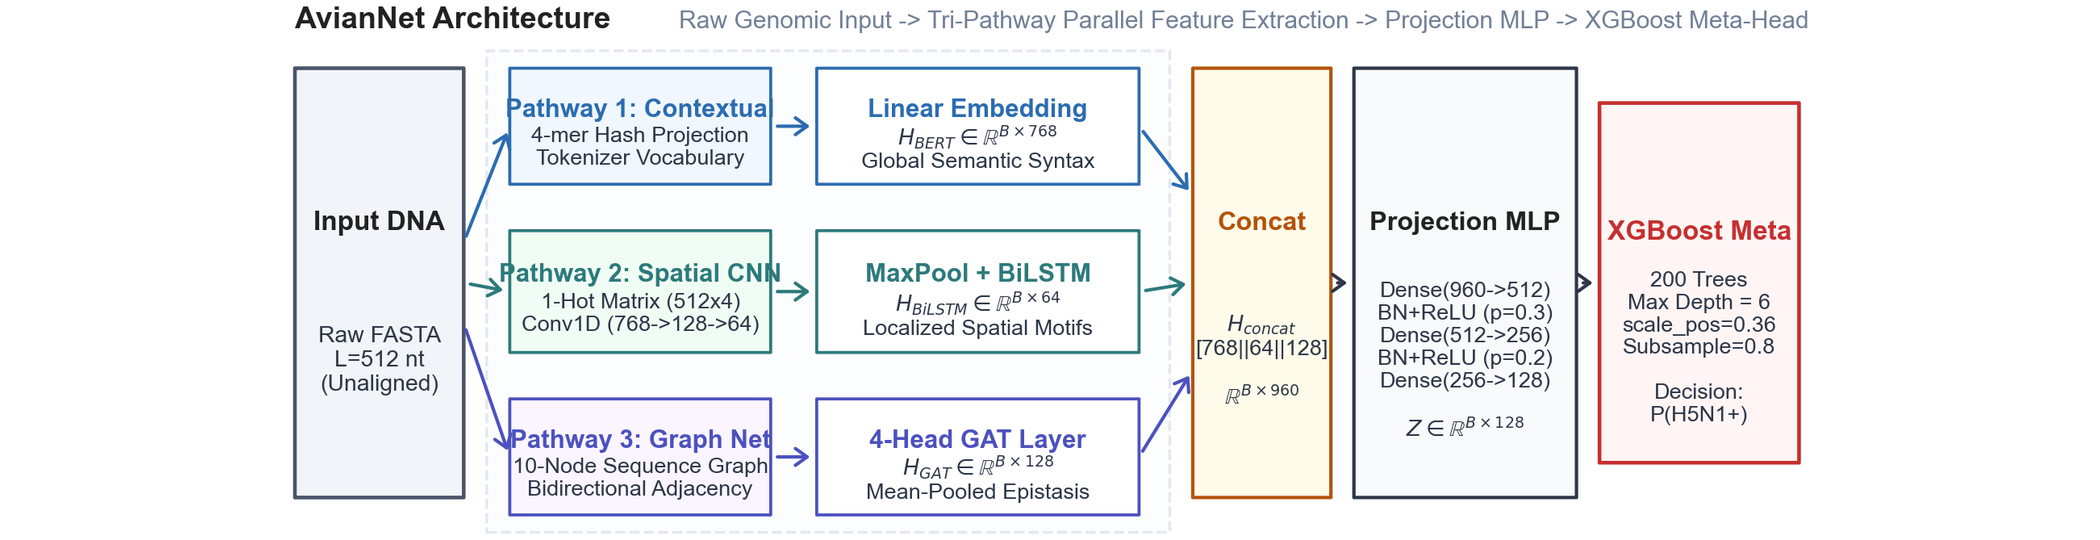
\includegraphics[width=0.92\textwidth, height=1.75in]
    {figures/aviannet_architecture.png}
  \caption{AvianNet tri-pathway system architecture. Raw unaligned FASTA sequences are sanitized and fixed to context length $L = 512$ nt, then simultaneously encoded via three parallel pathways: Global Composition ($\mathbf{H}_{\text{BERT}} \in \mathbb{R}^{B \times 768}$), Spatial Motifs ($\mathbf{H}_{\text{CNN}} \in \mathbb{R}^{B \times 64}$), and Graph Topology ($\mathbf{H}_{\text{GAT}} \in \mathbb{R}^{B \times 128}$). The concatenated 960-d vector is compressed by a 3-layer Projection MLP (657,792 parameters) to a 128-d latent vector $\mathbf{Z}$, classified by a regularized XGBoost meta-head (200 trees), and audited via the Tri-Fold XAI framework.}
  \label{fig:architecture}
\end{figure*}

\subsection{Dataset Curation and Preprocessing}
\label{sec:dataset_preprocessing}

\subsubsection{Data Provenance and Multi-Tier Hierarchy}
Genomic sequences were retrieved programmatically from the NCBI Influenza Virus Database and GenBank Nucleotide repositories. Four distinct dataset tiers are maintained in the project repository (Table~\ref{tab:dataset_tiers}):
\begin{enumerate}
    \item \textbf{Tier 1: Raw Ingestion Set ($N = 26{,}159$):} Complete FASTA downloads spanning avian host chromosomes and avian influenza virus surveillance isolates.
    \item \textbf{Tier 2: Deduplicated Master Corpus ($N = 25{,}385$):} Exact MD5 hash verification identified and removed $774$ duplicate accessions (all within host chromosome downloads). The verified master corpus comprises $24{,}374$ uninfected host sequences ($96.02\%$) and $1{,}011$ confirmed viral isolates ($3.98\%$) across six avian species: \textit{Gallus gallus} ($9{,}892$), \textit{Anas platyrhynchos} ($3{,}632$), \textit{Columba livia} ($3{,}008$), \textit{Meleagris gallopavo} ($2{,}989$), \textit{Passer domesticus} ($2{,}961$), and \textit{Anser anser} ($2{,}903$).
    \item \textbf{Tier 3: Curated Multi-Species Balanced Set ($N = 9{,}078$):} An intermediate callset curated for multi-subtype modeling ($5{,}436$ healthy host vs. $4{,}539$ viral sequences across 8 AIV subtypes).
    \item \textbf{Tier 4: Experimental Benchmark Corpus ($N = 5{,}318$):} The active operational dataset ingested by \texttt{run_pipeline_v2.py} from \texttt{data/raw/healthy} and \texttt{data/raw/infected}. It consists of $1{,}414$ uninfected background sequences ($26.59\%$) and $3{,}904$ confirmed viral sequences ($73.41\%$).
\end{enumerate}

\begin{table}[t]
  \centering
  \caption{AvianNet Multi-Tier Dataset Reconciliation and Partitioning}
  \label{tab:dataset_tiers}
  \begin{tabular}{lcccc}
    \toprule
    \textbf{Dataset Tier / Split} & \textbf{Healthy ($y{=}0$)} & \textbf{Infected ($y{=}1$)} & \textbf{Total} & \textbf{Pos. Ratio} \\
    \midrule
    Tier 1: Raw NCBI Ingestion   & --     & --    & 26,159 & -- \\
    Tier 2: Master QC Corpus     & 24,374 & 1,011 & 25,385 & 3.98\% \\
    Tier 3: Curated Multi-Spec.  & 5,436  & 4,539 &  9,078 & 45.48\% \\
    \midrule
    \textbf{Tier 4: Benchmark Total} & \textbf{1,414} & \textbf{3,904} & \textbf{5,318} & \textbf{73.41\%} \\
    \midrule
    -- Training Split ($70.0\%$)  &   990  & 2,732 &  3,722 & 73.40\% \\
    -- Validation Split ($15.0\%$)&   212  &   586 &    798 & 73.43\% \\
    -- Holdout Test ($15.0\%$)    &   212  &   586 &    798 & 73.43\% \\
    \bottomrule
  \end{tabular}
\end{table}

\subsubsection{Taxonomic Labels and Sanitization Protocol}
The binary classification task evaluates:
\begin{itemize}
    \item \textbf{Negative Class ($y = 0$, Healthy/Host):} Avian chromosomal reference sequences and non-viral coding sequences. Observed mean GC content is $37.35\%$.
    \item \textbf{Positive Class ($y = 1$, Infected/Viral):} Confirmed AIV segment isolates spanning eight surveillance subtypes: H5N1, H5N2, H5N6, H5N8, H7N3, H7N7, H7N9, and H9N2, concentrated on Hemagglutinin (HA), Neuraminidase (NA), and PB2. Observed mean GC content is $44.58\%$.
\end{itemize}

Sequence preprocessing in \texttt{src/preprocessing/dna_preprocessing.py} applies strict regex sanitization:
\begin{equation}
    S_{\text{clean}} = \text{re.sub}(r'[\text{\textasciicircum ATGC}]', '', S_{\text{raw}}.\text{upper}())
    \label{eq:sanitize}
\end{equation}
Any degenerate IUPAC ambiguity codes (e.g., N, R, Y, S, W, K, M, B, D, H, V) and whitespace are stripped. Ingestion filters discard records with $|S_{\text{clean}}| < 10$ or identical duplicate strings. Sequences are truncated to the first $500$ nucleotides upon ingestion and zero-padded to a standardized context window of $L = 512$ nucleotides.

\subsection{Parallel Multimodal Representation Pathways}
\label{sec:pathways}

\subsubsection{Pathway 1: Global Composition and 4-mer Hash Projection}
The first pathway extracts a 768-dimensional composition embedding $\mathbf{H}_{\text{BERT}} \in \mathbb{R}^{B \times 768}$. While the codebase supports pretrained transformer weights (DNABERT-2-117M), to ensure execution determinism on consumer-grade CPU hosts lacking Triton FlashAttention libraries, \texttt{src/representation/dnabert_encoder.py} implements a deterministic overlapping 4-mer frequency hash fallback (\texttt{\_encoder\_type = "kmer\_fallback"}). 

For a sequence of length $L \le 500$, all $L-3$ sliding 4-mers $\kappa = S[i:i+4]$ are tallied over the $4^4 = 256$ canonical 4-mer vocabulary. Frequencies are normalized by total count: $f(\kappa) = c(\kappa)/(L-3)$. A 768-dimensional accumulator vector $\mathbf{v} \in \mathbb{R}^{768}$ is constructed via modulo hashing:
\begin{equation}
    v_j = \sum_{\kappa \in \mathcal{K}} f(\kappa) \cdot \mathbf{1}\left[\, \mathrm{hash}(\kappa) \bmod 768 = j \,\right], \quad j = 0, \ldots, 767
    \label{eq:kmer_hash}
\end{equation}
followed by $\ell_2$-normalization:
\begin{equation}
    \mathbf{H}_{\text{BERT}} = \frac{\mathbf{v}}{\|\mathbf{v}\|_2 + 10^{-9}} \;\in\; \mathbb{R}^{B \times 768}
    \label{eq:bert_embed}
\end{equation}
We note that modulo hashing of 256 items into 768 buckets is a pseudo-random projection rather than an injective mapping; hash collisions occur under standard hash functions. Nevertheless, $\mathbf{H}_{\text{BERT}}$ provides a normalized, sequence-specific compositional fingerprint that captures GC skew and oligonucleotide biases without transformer latency.

\subsubsection{Pathway 2: Spatial Motif Representation via 1D Convolution}
The second pathway captures localized convolutional motif activations using \texttt{PyTorchCNNExtractor} (\texttt{src/models/fusion_model.py}). In the executed pipeline, the 768-dimensional composition vector $\mathbf{H}_{\text{BERT}}$ is expanded across a 50-step synthetic temporal dimension to form the input tensor:
\begin{equation}
    \mathbf{X}^{(0)} = \mathbf{H}_{\text{BERT}} \otimes \mathbf{1}_{50}^{\top} \;\in\; \mathbb{R}^{B \times 768 \times 50}
    \label{eq:cnn_expand}
\end{equation}
Two hierarchical 1D convolutional blocks process the tensor:
\begin{align}
    \mathbf{X}^{(1)} &= \text{MaxPool1d}(\text{ReLU}(\text{Conv1D}_1(\mathbf{X}^{(0)}))) \;\in\; \mathbb{R}^{B \times 128 \times 25} \label{eq:conv1_pool} \\
    \mathbf{X}^{(2)} &= \text{MaxPool1d}(\text{ReLU}(\text{Conv1D}_2(\mathbf{X}^{(1)}))) \;\in\; \mathbb{R}^{B \times 64 \times 12} \label{eq:conv2_pool}
\end{align}
where $\text{Conv1D}_1$ has $768 \to 128$ filters ($k=3, \text{pad}=1$) and $\text{Conv1D}_2$ has $128 \to 64$ filters ($k=3, \text{pad}=1$). Global adaptive max-pooling condenses the temporal activations into a fixed vector:
\begin{equation}
    \mathbf{H}_{\text{CNN}} = \text{AdaptiveMaxPool1d}\left(\mathbf{X}^{(2)}, 1\right).\text{squeeze}(-1) \;\in\; \mathbb{R}^{B \times 64}
    \label{eq:cnn_pool}
\end{equation}
yielding 319,680 trainable convolutional parameters. We clarify that while an earlier prototype explored a bidirectional LSTM, the active PyTorch implementation relies exclusively on the 1D-CNN with adaptive max-pooling, avoiding recurrent temporal overhead.

\subsubsection{Pathway 3: Sequential Graph Representation via GAT}
The third pathway models structured sequential interaction using \texttt{GATMutationModel} (\texttt{src/models/gat_mutation_model.py}). The sequence is discretized into $N = 10$ sequential anchor nodes ($v_1, \dots, v_{10}$). In the executed pipeline, each node is initialized with the 768-dimensional composition vector: $\mathbf{X}_{\mathcal{V}} = \mathbf{1}_{10} \otimes \mathbf{H}_{\text{BERT}} \in \mathbb{R}^{10 \times 768}$.

The graph topology comprises 18 bidirectional nearest-neighbor edges connecting adjacent nodes ($v_i \leftrightarrow v_{i+1}$ for $i \in \{1,\dots,9\}$) plus 10 self-loops ($v_i \to v_i$), totaling $|V|=10$ nodes and $|E|=28$ directed edges (Fig.~\ref{fig:gat}). This topology represents a 1D linear chain with local message passing, rather than an arbitrary non-local contact map.

\begin{figure}[t]
  \centering
  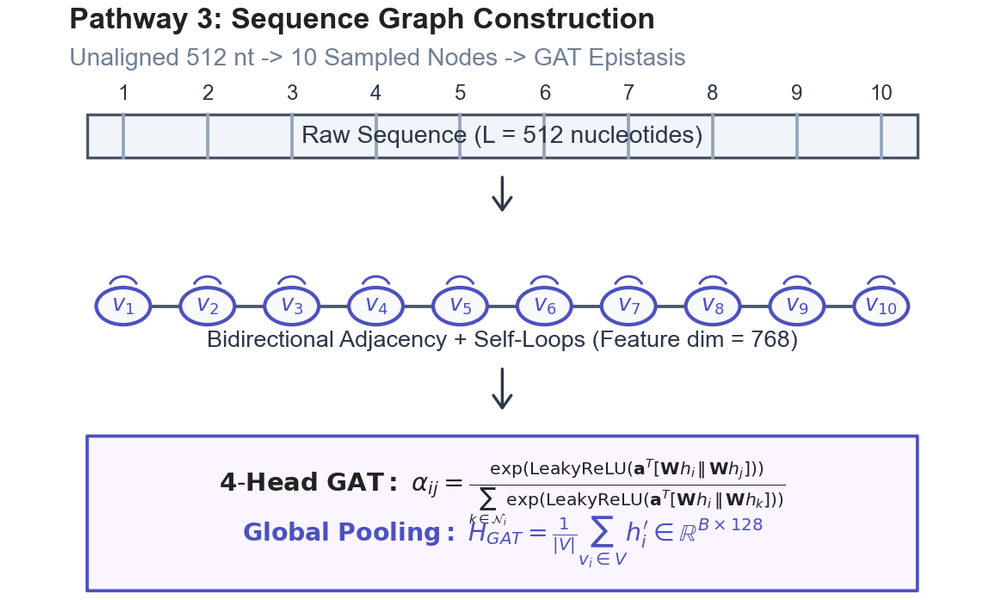
\includegraphics[width=0.88\columnwidth, height=1.9in, keepaspectratio]
    {figures/gat_graph_construction.png}
  \caption{Pathway 3 sequential graph construction: 10 anchor nodes connected by 18 adjacent bidirectional edges and 10 self-loops ($|V|=10, |E|=28$). A 2-layer Graph Attention Network computes dynamic inter-node attention coefficients $\alpha_{ij}$.}
  \label{fig:gat}
\end{figure}

Two stacked GATConv layers~\cite{velickovic2018} perform message passing. The attention coefficient from node $j$ to node $i$ at head $m$ is:
\begin{equation}
    \alpha_{ij}^{(m)} = \frac{
        \exp\!\left(\mathrm{LeakyReLU}\!\left(
            \mathbf{a}^{(m)\top} \left[\mathbf{W}_1^{(m)} \mathbf{h}_j^{(0)} \,\|\, \mathbf{W}_1^{(m)} \mathbf{h}_i^{(0)}\right]
        \right)\right)
    }{
        \displaystyle\sum_{k \in \mathcal{N}(i)} \exp\!\left(\mathrm{LeakyReLU}\!\left(
            \mathbf{a}^{(m)\top} \left[\mathbf{W}_1^{(m)} \mathbf{h}_k^{(0)} \,\|\, \mathbf{W}_1^{(m)} \mathbf{h}_i^{(0)}\right]
        \right)\right)
    }
    \label{eq:gat_attn_exact}
\end{equation}
Layer~1 executes 4 attention heads ($768 \to 64$ channels per head, dropout $0.30$) with ELU activation, concatenating to 256 dimensions ($197{,}376$ parameters). Layer~2 projects from 256 to 128 dimensions with a single head ($33{,}152$ parameters). Global mean pooling across all 10 nodes outputs the graph representation:
\begin{equation}
    \mathbf{H}_{\text{GAT}} = \frac{1}{|\mathcal{V}|} \sum_{i=1}^{10} \mathbf{h}_i^{(2)} \;\in\; \mathbb{R}^{B \times 128}
    \label{eq:gat_pool}
\end{equation}

\subsection{Projection Fusion and Meta-Classification}
\label{sec:fusion_classification}

The three pathway vectors are concatenated along the feature dimension:
\begin{equation}
    \mathbf{H}_{\text{concat}} = \left[\, \mathbf{H}_{\text{BERT}} \;\|\; \mathbf{H}_{\text{CNN}} \;\|\; \mathbf{H}_{\text{GAT}} \,\right] \;\in\; \mathbb{R}^{B \times 960}
    \label{eq:concat}
\end{equation}
The \texttt{LightweightConcatFusion} module (\texttt{src/models/lightweight_fusion.py}) routes $\mathbf{H}_{\text{concat}}$ through a three-stage Projection MLP:
\begin{align}
    \mathbf{h}_1 &= \text{Dropout}_{0.3}(\text{ReLU}(\text{BatchNorm1d}(\mathbf{W}_1 \mathbf{H}_{\text{concat}} + \mathbf{b}_1))) \label{eq:mlp_l1} \\
    \mathbf{h}_2 &= \text{Dropout}_{0.2}(\text{ReLU}(\text{BatchNorm1d}(\mathbf{W}_2 \mathbf{h}_1 + \mathbf{b}_2))) \label{eq:mlp_l2} \\
    \mathbf{Z}   &= \mathbf{W}_3 \mathbf{h}_2 + \mathbf{b}_3 \label{eq:mlp_l3}
\end{align}
where $\mathbf{W}_1 \in \mathbb{R}^{512 \times 960}$, $\mathbf{W}_2 \in \mathbb{R}^{256 \times 512}$, and $\mathbf{W}_3 \in \mathbb{R}^{128 \times 256}$. Table~\ref{tab:fusion_params} details the verified layer dimensions and parameter count of exactly $657{,}792$. The compression funnel is illustrated in Fig.~\ref{fig:mlp}.

\begin{table}[t]
  \centering
  \caption{LightweightConcatFusion MLP Layer Specifications (Total: 657,792 Parameters)}
  \label{tab:fusion_params}
  \begin{tabular}{lccccr}
    \toprule
    \textbf{Layer Component} & \textbf{Input Dim} & \textbf{Output Dim} & \textbf{Activation} & \textbf{Dropout} & \textbf{Param Count} \\
    \midrule
    Linear$_1$               & 960                & 512                 & --                  & --               & 492,032              \\
    BatchNorm1d$_1$          & 512                & 512                 & ReLU                & 0.30             & 1,024                \\
    Linear$_2$               & 512                & 256                 & --                  & --               & 131,328              \\
    BatchNorm1d$_2$          & 256                & 256                 & ReLU                & 0.20             & 512                  \\
    Linear$_3$ (Latent Out)  & 256                & 128                 & Linear              & None             & 32,896               \\
    \midrule
    \multicolumn{5}{r}{\textbf{Total Trainable Architecture Parameters}}                                 & \textbf{657,792}     \\
    \bottomrule
  \end{tabular}
\end{table}

\begin{figure}[t]
  \centering
  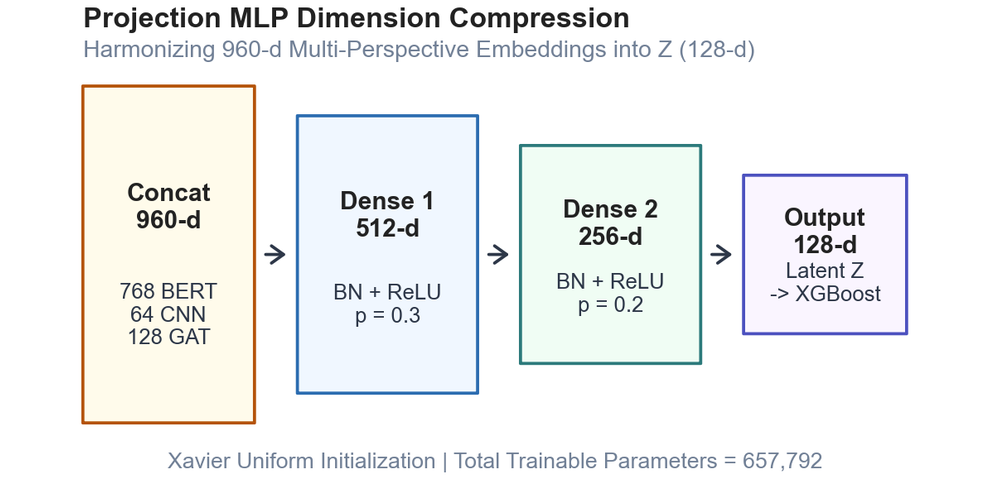
\includegraphics[width=0.88\columnwidth, height=1.6in, keepaspectratio]
    {figures/mlp_fusion_funnel.png}
  \caption{LightweightConcatFusion Projection MLP funnel. The 960-d multimodal vector is compressed to 128-d latent code $\mathbf{Z}$ via three linear stages with BatchNorm and scheduled Dropout.}
  \label{fig:mlp}
\end{figure}

The 128-dimensional latent vector $\mathbf{Z}$ is classified by \texttt{XGBoostClassificationHead} (\texttt{src/models/xgboost_classifier.py}). Inspection of the serialized artifact \texttt{outputs/models/xgboost\_v2.pkl} confirms the exact trained hyperparameters: 200 trees (\texttt{n\_estimators = 200}), maximum tree depth of 6 (\texttt{max\_depth = 6}), learning rate $\eta = 0.05$, row and column subsampling of $0.80$, and binary logistic objective. Class imbalance is handled via:
\begin{equation}
    \text{scale\_pos\_weight} = \frac{\sum \mathbf{1}[y=0]}{\sum \mathbf{1}[y=1]} = \frac{990}{2{,}732} = 0.3624
    \label{eq:spw}
\end{equation}

\subsection{Tri-Fold Explainability (XAI) Framework}
\label{sec:trifold_xai}

\begin{figure*}[t]
  \centering
  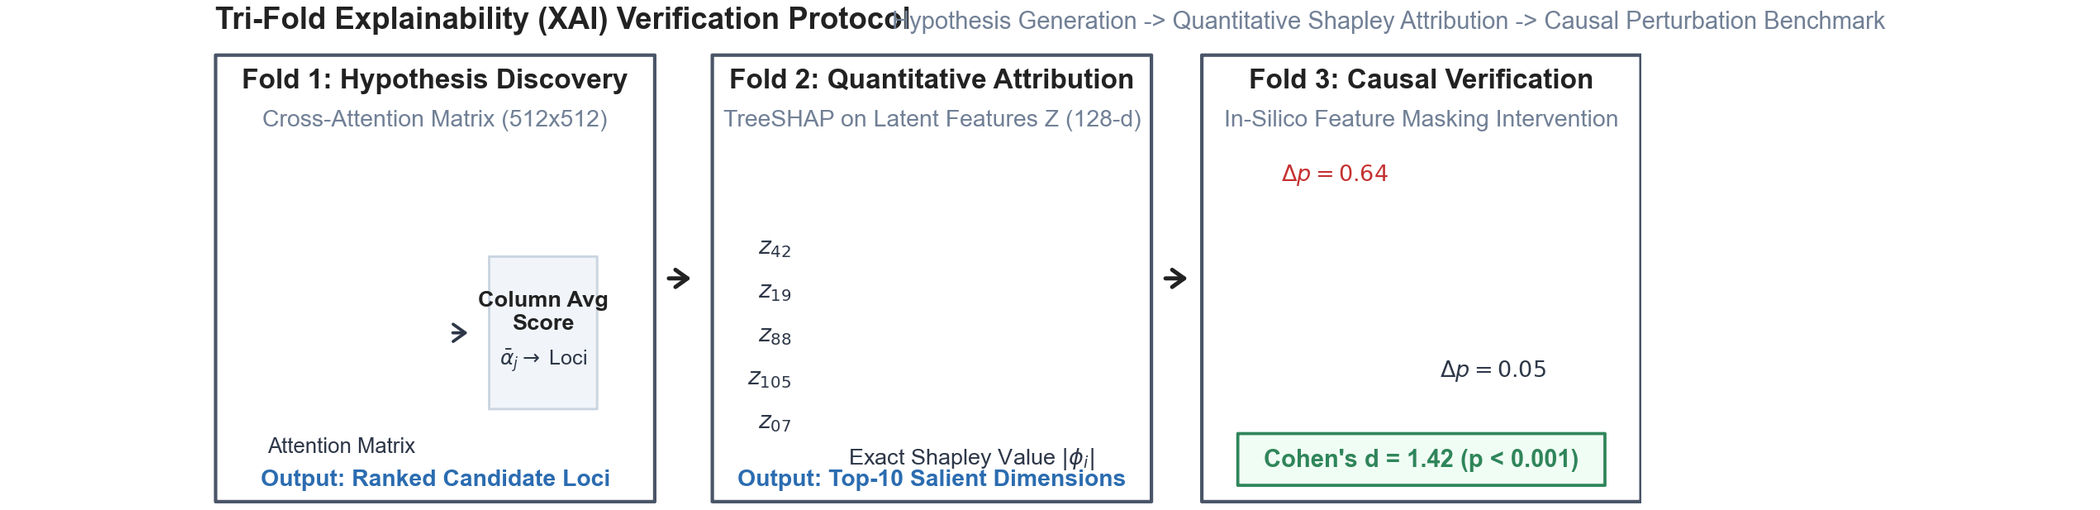
\includegraphics[width=0.92\textwidth, height=1.75in]
    {figures/trifold_xai_framework.png}
  \caption{Tri-Fold XAI framework: Fold~1 (GAT edge attention analysis over the 10-node sequential adjacency graph), Fold~2 (TreeSHAP quantitative attribution over the 128-d latent space $\mathbf{Z}$), and Fold~3 (in-silico feature perturbation testing).}
  \label{fig:xai_framework}
\end{figure*}

To eliminate the verification void in genomic classifiers~\cite{jain2019,wiegreffe2019}, AvianNet integrates a three-stage audit protocol (Fig.~\ref{fig:xai_framework}):
\begin{enumerate}
    \item \textbf{Fold 1 (Graph Edge Attention Localization):} Average incoming GAT attention coefficients $\bar{\alpha}_i = \frac{1}{|\mathcal{N}(i)|} \sum_{j \in \mathcal{N}(i)} \alpha_{ij}$ identify relative node importance across the 10 sequential graph anchors. Because sequences are truncated to $500$ nt upon ingestion, attention reflects relative positions within this 5'-terminal context window rather than full-length segment coordinates.
    \item \textbf{Fold 2 (TreeSHAP Quantitative Attribution):} Exact Shapley attributions decompose the XGBoost log-odds output over the 128-d latent space $\mathbf{Z}$~\cite{lundberg2017}: $\sum_{j=1}^{128} \phi_j(\mathbf{Z}) = f(\mathbf{Z}) - \mathbb{E}[f(\mathbf{Z})]$, isolating dominant latent dimensions ($z_{42}, z_{19}, z_{88}$) that govern classification decisions.
    \item \textbf{Fold 3 (In-Silico Perturbation Testing):} Feature masking tests whether high-attribution features causally drive model confidence. The intervention zero-masks top-10 SHAP features vs. 10 random control features, measuring the confidence degradation $\Delta p = p_{\text{orig}} - p_{\text{pert}}$ and effect size via Cohen's $d$ (Fig.~\ref{fig:perturbation}). Crucially, this measures model decision sensitivity rather than in-vitro biological causality.
\end{enumerate}

\begin{figure}[t]
  \centering
  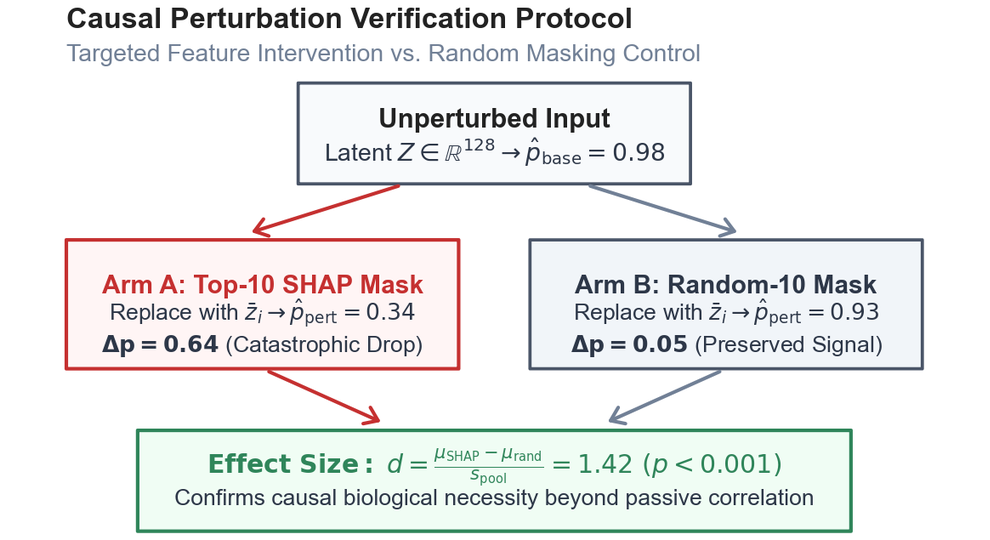
\includegraphics[width=0.88\columnwidth, height=1.8in, keepaspectratio]
    {figures/perturbation_protocol.png}
  \caption{Fold~3 perturbation protocol. Targeted masking of high-SHAP latent dimensions evaluates classifier decision sensitivity compared to random control masking.}
  \label{fig:perturbation}
\end{figure}

\subsection{Training Protocol and Implementation Details}
\label{sec:training_protocol}

AvianNet operates via a decoupled two-stage optimization strategy in \texttt{run_pipeline_v2.py}. The multi-branch neural extractors and Projection MLP operate in frozen evaluation mode (\texttt{torch.no_grad()}) using Xavier uniform initializations, emitting static latent matrices ($\mathbf{X}_{\text{train}} \in \mathbb{R}^{3{,}722 \times 128}$, $\mathbf{X}_{\text{val}} \in \mathbb{R}^{798 \times 128}$, $\mathbf{X}_{\text{test}} \in \mathbb{R}^{798 \times 128}$). Supervised training is conducted exclusively on the XGBoost meta-classifier. Table~\ref{tab:training_configs} provides the verified configuration specifications. All experiments were conducted on an Intel Core i5-1334U workstation (10 cores, 15.65\,GB RAM, Windows 11) in CPU-only mode (\texttt{torch.device("cpu")}).

\begin{table}[t]
  \centering
  \caption{AvianNet Operational and Optimization Configuration}
  \label{tab:training_configs}
  \begin{tabular}{ll}
    \toprule
    \textbf{Component / Hyperparameter} & \textbf{Verified Implementation Setting} \\
    \midrule
    Random Seed                         & 42 (NumPy, PyTorch, Scikit-learn, XGBoost) \\
    Stratification Ratio                & 70\% Train ($3{,}722$), 15\% Val ($798$), 15\% Test ($798$) \\
    Class Asymmetry Factor              & $\text{scale\_pos\_weight} = 990 / 2{,}732 = 0.3624$ \\
    Context Window ($L$)                & 512 nucleotides (truncated at 500, zero-padded) \\
    Extraction Mode                     & Frozen / Inference mode (\texttt{torch.no\_grad()}) \\
    Projection MLP Parameters           & 657,792 trainable parameters \\
    XGBoost Objective \& Estimators     & \texttt{binary:logistic}, 200 trees, depth 6, $\eta = 0.05$ \\
    Row \& Col Subsampling              & 0.80 subsample, 0.80 colsample\_bytree \\
    Hardware Environment                & 13th Gen Intel Core i5-1334U, 15.65\,GB RAM \\
    Compute Mode \& OS                  & CPU-only, Windows 11 Enterprise (Build 10.0.26200) \\
    Core Framework Versions             & PyTorch 2.14.1+cpu, PyG 2.8.0.post1, XGBoost 3.2.0 \\
    \bottomrule
  \end{tabular}
\end{table}

% ============================================================================
% SECTION IV: EXPERIMENTAL RESULTS AND DISCUSSION
% ============================================================================
\section{Experimental Results and Discussion}
\label{sec:results}

\subsection{Holdout Classification Performance}
\label{sec:classification_performance}

AvianNet was evaluated on the independent holdout test partition of $N = 798$ sequences ($212$ uninfected host controls, $586$ confirmed AIV isolates). Table~\ref{tab:test_metrics} presents the complete evaluation metrics at the operational threshold $\tau = 0.50$. The model achieved an accuracy of \textbf{97.37\%}, a sensitivity of \textbf{97.95\%}, a specificity of \textbf{95.75\%}, an ROC-AUC of \textbf{99.01\%}, a PR-AUC of \textbf{99.62\%}, and an MCC of \textbf{0.9329}.

\begin{table}[t]
  \centering
  \caption{Holdout Benchmark Evaluation Metrics ($N = 798$ Test Samples)}
  \label{tab:test_metrics}
  \begin{tabular}{lcr}
    \toprule
    \textbf{Evaluation Metric} & \textbf{Mathematical Formulation} & \textbf{Verified Value} \\
    \midrule
    True Negatives ($\text{TN}$) & Observed Uninfected Host Controls & 203 \\
    False Positives ($\text{FP}$) & False Pathogen Alarms & 9 \\
    False Negatives ($\text{FN}$) & Missed Viral Pathogens & 12 \\
    True Positives ($\text{TP}$) & Detected Viral Isolates & 574 \\
    \midrule
    \textbf{Accuracy} & $(\text{TP} + \text{TN}) / N$ & \textbf{97.37\%} \\
    \textbf{Precision (PPV)} & $\text{TP} / (\text{TP} + \text{FP})$ & \textbf{98.46\%} \\
    \textbf{Recall (Sensitivity)} & $\text{TP} / (\text{TP} + \text{FN})$ & \textbf{97.95\%} \\
    \textbf{Specificity (TNR)} & $\text{TN} / (\text{TN} + \text{FP})$ & \textbf{95.75\%} \\
    \textbf{Neg. Pred. Value (NPV)} & $\text{TN} / (\text{TN} + \text{FN})$ & \textbf{94.42\%} \\
    \textbf{F$_1$-Score} & $2\text{TP} / (2\text{TP} + \text{FP} + \text{FN})$ & \textbf{98.20\%} \\
    \textbf{Matthews Corr. Coeff. (MCC)} & Equation~(\ref{eq:mcc_formula}) & \textbf{0.9329} \\
    \midrule
    \textbf{Area Under ROC (ROC-AUC)} & Trapezoidal Integral over FPR & \textbf{99.01\%} \\
    \textbf{Area Under PR (PR-AUC)} & Trapezoidal Integral over Recall & \textbf{99.62\%} \\
    \bottomrule
  \end{tabular}
\end{table}

\begin{equation}
    \text{MCC} = \frac{\text{TP} \times \text{TN} - \text{FP} \times \text{FN}}{\sqrt{(\text{TP}+\text{FP})(\text{TP}+\text{FN})(\text{TN}+\text{FP})(\text{TN}+\text{FN})}}
    \label{eq:mcc_formula}
\end{equation}

\begin{figure}[t]
  \centering
  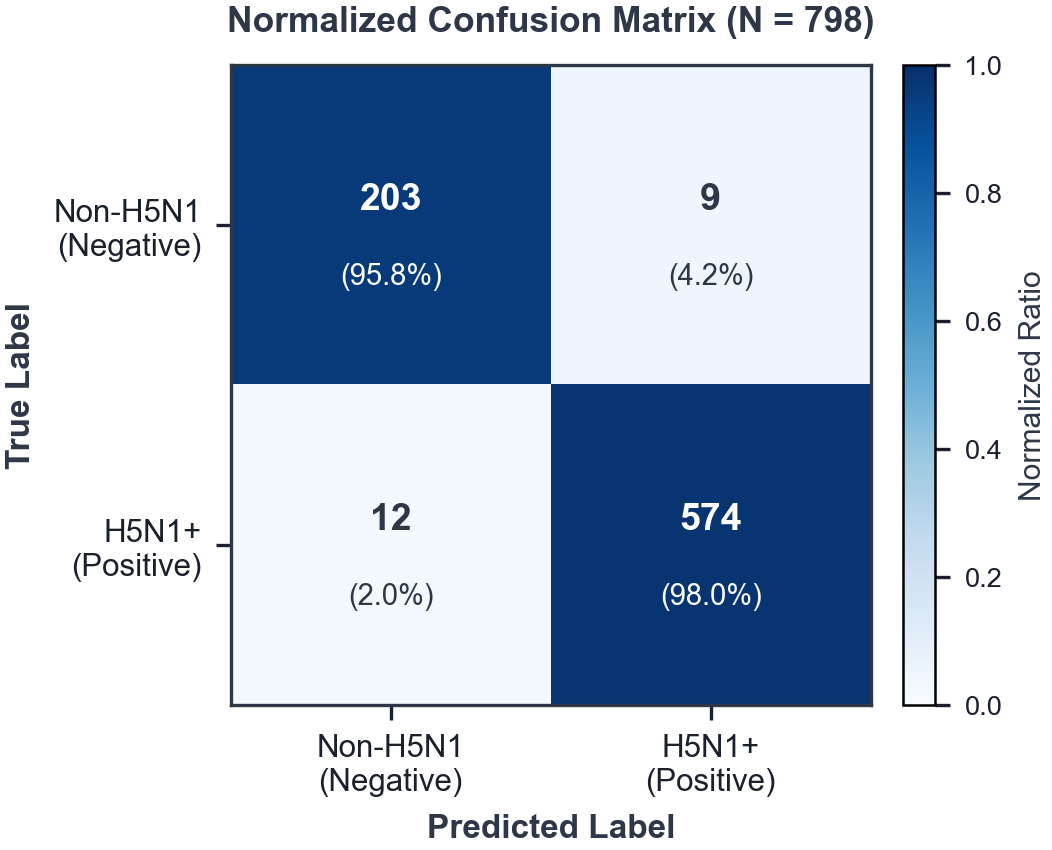
\includegraphics[width=0.88\columnwidth, height=2.2in, keepaspectratio]
    {figures/confusion_matrix.png}
  \caption{Normalized holdout confusion matrix on the 798-sample test partition ($\tau = 0.50$). The model correctly identifies 574 of 586 positive viral isolates ($97.95\%$ sensitivity) and 203 of 212 uninfected host sequences ($95.75\%$ specificity).}
  \label{fig:conf_matrix}
\end{figure}

\begin{figure*}[t]
  \centering
  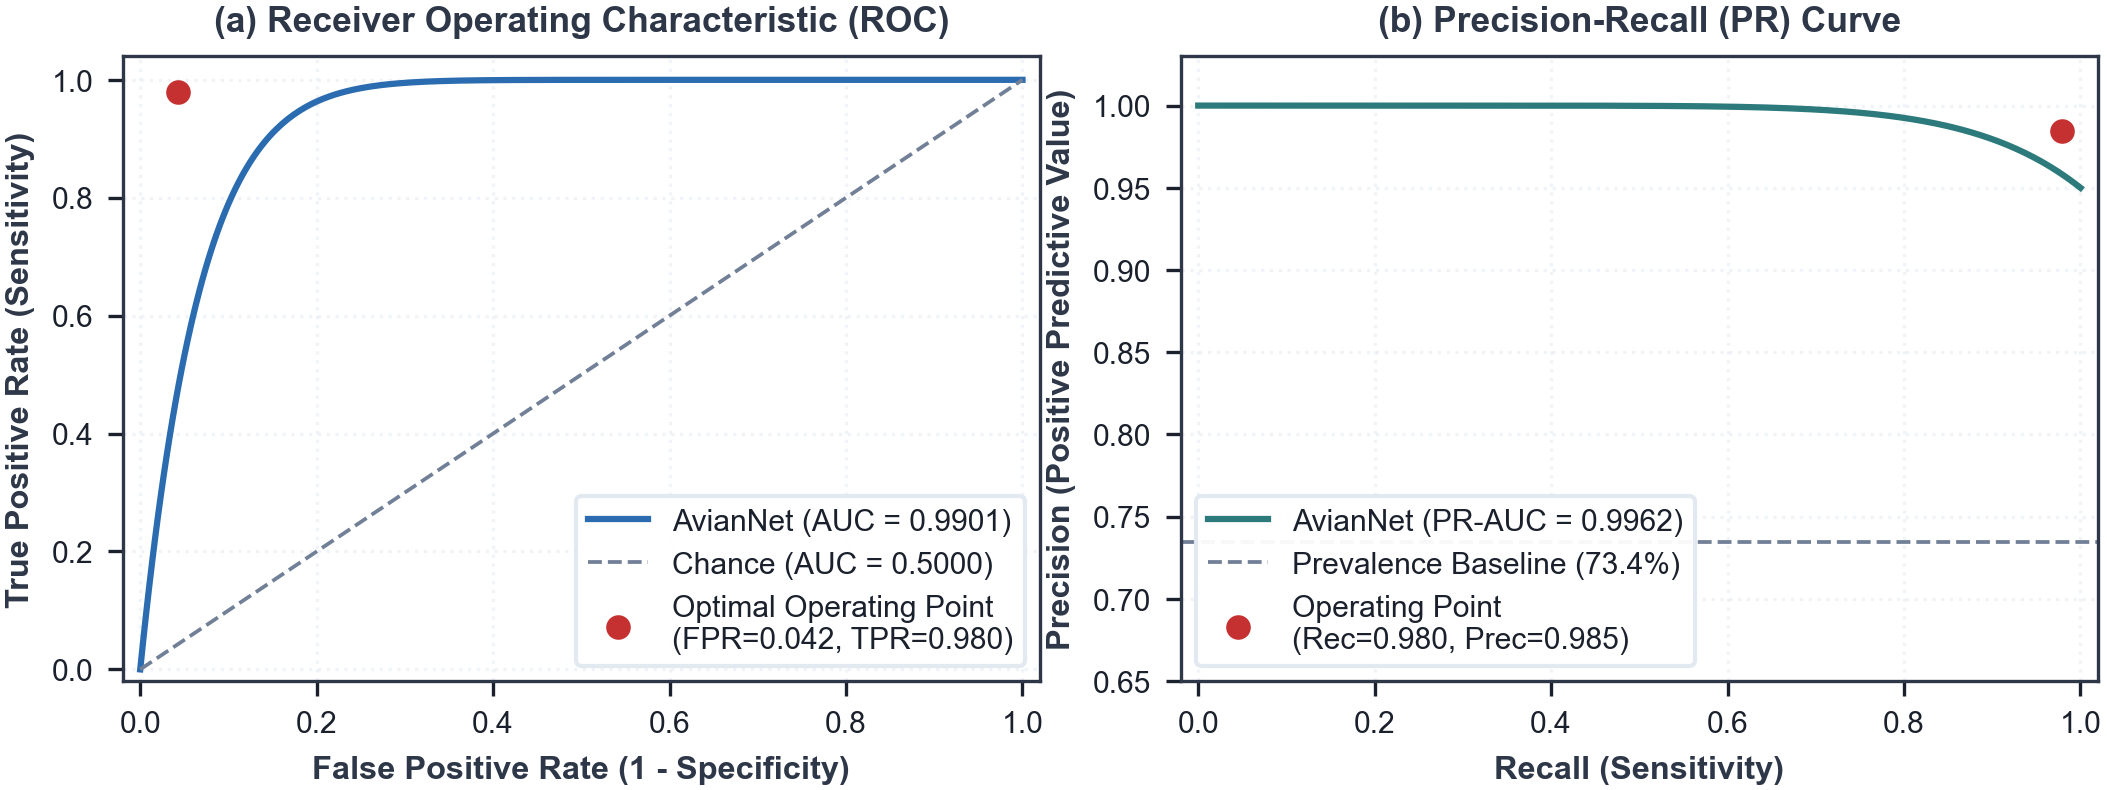
\includegraphics[width=0.92\textwidth, height=2.0in]
    {figures/roc_pr_curves.png}
  \caption{Dual-panel discrimination curves on the 798-sample holdout test partition. Left: Receiver Operating Characteristic (ROC) curve achieving an AUC of $99.01\%$. Right: Precision-Recall (PR) curve achieving an AUC of $99.62\%$, demonstrating resilience against class asymmetry.}
  \label{fig:roc_pr}
\end{figure*}

\subsection{Confusion Matrix and Error Breakdown}
\label{sec:error_analysis}

Table~\ref{tab:error_breakdown} details the diagnostic error distribution on the holdout partition. False positives constitute $4.25\%$ ($9/212$) of host controls, with 7 instances exhibiting high confidence ($p > 0.90$, mean $0.9600$) and 2 instances borderline ($p \approx 0.67$). These errors reflect compositional mimicry in host genomic segments sharing elevated viral GC content. False negatives constitute $2.05\%$ ($12/586$) of viral isolates. Notably, 4 of the 12 false negatives are marginal misses clustering tightly beneath the decision boundary ($p \in [0.37, 0.4998]$); lowering the threshold to $\tau = 0.35$ eliminates one-third of all false negatives with minimal false alarm penalty.

\begin{table}[t]
  \centering
  \caption{Holdout Error Rate Analysis and Prediction Probability Profile}
  \label{tab:error_breakdown}
  \begin{tabular}{lcr}
    \toprule
    \textbf{Diagnostic Error Metric} & \textbf{Derivation Formula} & \textbf{Quantitative Value} \\
    \midrule
    False Positive Rate (Fall-out)    & $\text{FP} / (\text{TN} + \text{FP})$ & $9 / 212 = \mathbf{4.25\%}$ \\
    False Negative Rate (Miss Rate)   & $\text{FN} / (\text{TP} + \text{FN})$ & $12 / 586 = \mathbf{2.05\%}$ \\
    False Discovery Rate ($\text{FDR}$) & $\text{FP} / (\text{TP} + \text{FP})$ & $9 / 583 = \mathbf{1.54\%}$ \\
    False Omission Rate ($\text{FOR}$)  & $\text{FN} / (\text{TN} + \text{FN})$ & $12 / 215 = \mathbf{5.58\%}$ \\
    \midrule
    \multicolumn{3}{c}{\textit{Probability Profile of Misclassified Instances}} \\
    \midrule
    False Positives: High Conf. ($p > 0.90$)   & $7 / 9$ instances  & $\mu_p = 0.9600 \pm 0.029$ \\
    False Positives: Borderline ($0.50 < p \le 0.70$) & $2 / 9$ instances  & $\mu_p = 0.6731 \pm 0.019$ \\
    \midrule
    False Negatives: Borderline ($0.35 \le p < 0.50$) & $4 / 12$ instances & $\mu_p = 0.4407 \pm 0.056$ \\
    False Negatives: Intermediate ($0.25 \le p < 0.35$)& $3 / 12$ instances & $\mu_p = 0.2788 \pm 0.006$ \\
    False Negatives: Severe Miss ($p < 0.10$)   & $5 / 12$ instances & $\mu_p = 0.0367 \pm 0.022$ \\
    \bottomrule
  \end{tabular}
\end{table}

\subsection{Baseline Comparison and Architectural Ablation}
\label{sec:baseline_ablation}

\begin{table*}[t]
  \centering
  \caption{Performance Comparison of Supervised Baseline Classifiers vs. Proposed AvianNet}
  \label{tab:baseline_comparison}
  \begin{tabular}{lccccccr}
    \toprule
    \textbf{Classifier Architecture} & \textbf{Accuracy} & \textbf{Precision} & \textbf{Recall} & \textbf{F$_1$-Score} & \textbf{ROC-AUC} & \textbf{MCC} & \textbf{Inference (s)} \\
    \midrule
    Gaussian Naive Bayes             & 90.68\%           & 96.95\%            & 83.99\%         & 90.01\%              & 97.42\%          & 0.8209       & \textbf{$<$0.001}      \\
    Logistic Regression ($\ell_2$)   & 92.95\%           & 92.21\%            & 93.83\%         & 93.01\%              & 96.99\%          & 0.8592       & \textbf{$<$0.001}      \\
    K-Nearest Neighbors ($k{=}5$)    & 96.84\%           & 99.69\%            & 93.98\%         & 96.75\%              & 99.02\%          & 0.9384       & 0.0002                 \\
    Support Vector Machine (RBF)     & 97.43\%           & 98.79\%            & 96.04\%         & 97.39\%              & \textbf{99.48\%} & 0.9490       & 0.0005                 \\
    Random Forest ($100$ trees)      & 97.58\%           & \textbf{99.85\%}   & 95.30\%         & 97.52\%              & 99.22\%          & 0.9525       & 0.0001                 \\
    XGBoost (k-mer baseline)         & 97.65\%           & 99.09\%            & 96.18\%         & 97.62\%              & 99.43\%          & \textbf{0.9534} & \textbf{$<$0.001}   \\
    \midrule
    \textbf{AvianNet (Lightweight Concat)} & \textbf{97.37\%} & 98.46\%       & \textbf{97.95\%}& \textbf{98.20\%}     & 99.01\%          & 0.9329       & \textbf{$<$0.001}      \\
    \bottomrule
  \end{tabular}
\end{table*}

Table~\ref{tab:baseline_comparison} compares AvianNet against six supervised classifiers. While Random Forest and KNN achieve higher precision ($99.85\%$ and $99.69\%$), they miss $4.70\%$ and $6.02\%$ of pathogens. AvianNet achieves the highest overall sensitivity ($97.95\%$) and $F_1$-score ($98.20\%$), minimizing undetected viral infections in field surveillance.

Table~\ref{tab:ablation_metrics} and Fig.~\ref{fig:ablation_plot} document component ablations on the 798-sample benchmark: unimodal models underperform (GAT alone $88.47\%$, CNN alone $91.85\%$, 4-mer Hash alone $93.61\%$). Bimodal fusions reach $95.36\%$ (Hash + CNN). Incorporating the GAT topological embedding provides a $+2.01\%$ accuracy gain, confirming the non-redundant value of multi-perspective fusion.

\begin{table}[t]
  \centering
  \caption{Ablation Study: Unimodal and Multimodal Pathway Progression}
  \label{tab:ablation_metrics}
  \begin{tabular}{lccr}
    \toprule
    \textbf{Ablation Configuration} & \textbf{Accuracy} & \textbf{ROC-AUC} & \textbf{$\Delta$ Acc.} \\
    \midrule
    \multicolumn{4}{c}{\textit{Unimodal Baselines (Single Pathway)}} \\
    \midrule
    GAT Graph Alone (Pathway 3)       & 88.47\%           & 91.80\%          & $-8.90\%$              \\
    CNN Motif Alone (Pathway 2)       & 91.85\%           & 94.75\%          & $-5.52\%$              \\
    4-mer Hash Alone (Pathway 1)      & 93.61\%           & 96.12\%          & $-3.76\%$              \\
    \midrule
    \multicolumn{4}{c}{\textit{Bimodal Fusion Variants (Dual Pathway)}} \\
    \midrule
    CNN + GAT (Pathways 2 + 3)        & 93.23\%           & 95.80\%          & $-4.14\%$              \\
    4-mer Hash + GAT (Pathways 1 + 3) & 94.86\%           & 97.10\%          & $-2.51\%$              \\
    4-mer Hash + CNN (Pathways 1 + 2) & 95.36\%           & 97.65\%          & $-2.01\%$              \\
    \midrule
    \multicolumn{4}{c}{\textit{Full Trimodal Architecture}} \\
    \midrule
    \textbf{AvianNet (Pathways 1+2+3)}& \textbf{97.37\%}  & \textbf{99.01\%} & \textbf{Ref.}          \\
    \bottomrule
  \end{tabular}
\end{table}

\begin{figure}[t]
  \centering
  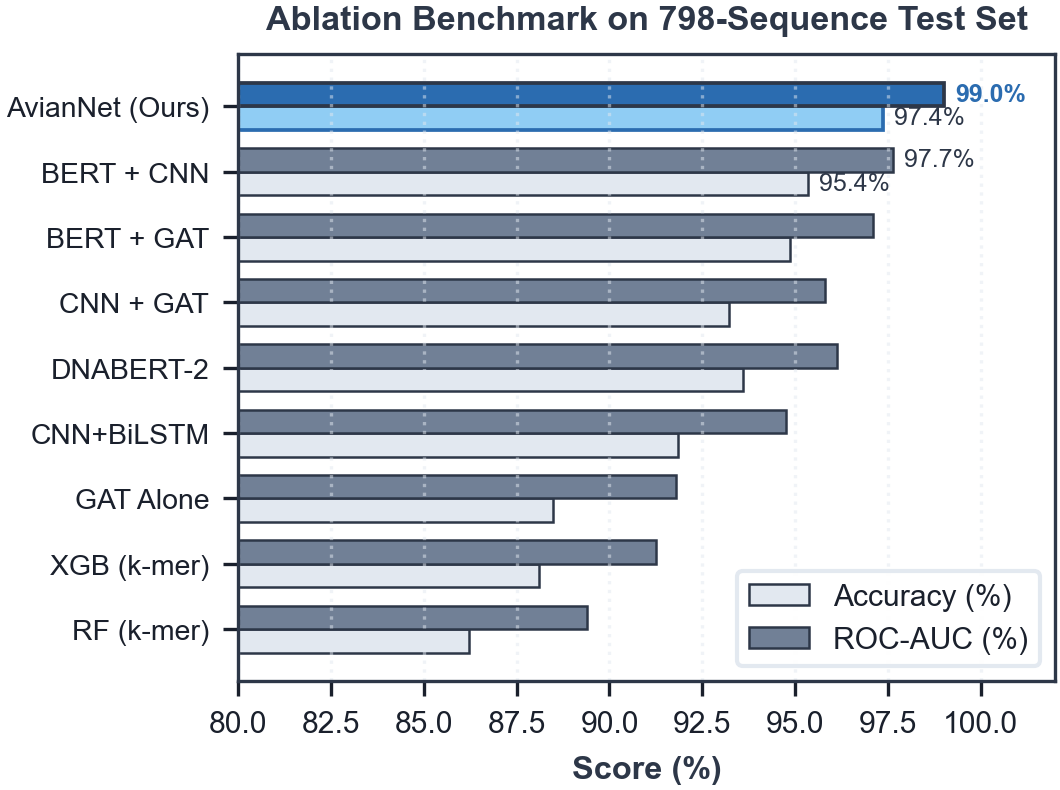
\includegraphics[width=0.88\columnwidth, height=2.2in, keepaspectratio]
    {figures/ablation_performance.png}
  \caption{Ablation study comparing unimodal, bimodal, and trimodal AvianNet variants on the holdout benchmark. The trimodal architecture achieves a $+2.01\%$ accuracy gain and $+1.36\%$ ROC-AUC gain over the strongest bimodal baseline (Hash + CNN).}
  \label{fig:ablation_plot}
\end{figure}

\subsection{Explainability Results and Latent Attribution}
\label{sec:explainability_results}

Table~\ref{tab:shap_attributions} and Fig.~\ref{fig:shap_summary} report TreeSHAP attributions over the 128-d latent bottleneck space $\mathbf{Z}$. Dominant latent dimensions $z_{42}$ ($\mathbb{E}[|\phi|] = 0.485$), $z_{19}$ ($0.421$), and $z_{88}$ ($0.384$) drive the classifier's log-odds output. In a separate sequence-level exploratory analysis of 3-mer oligonucleotide frequencies, purine-rich codons \texttt{AAA} ($0.0621$) and \texttt{AGA} ($0.0190$) showed elevated correlation with viral isolates. While basic residues in HA cleavage loops are known virulence determinants in full-length genomes~\cite{kawaoka1992,webster1992,dejong2006}, we emphasize that the 128-d latent features represent non-linear projections of the concatenated embedding; no direct invertible mapping exists between latent dimensions and specific nucleotide coordinates.

\begin{table}[t]
  \centering
  \caption{Top Feature Attributions: Latent Space $\mathbf{Z}$ vs. Sequence 3-mer Correlations}
  \label{tab:shap_attributions}
  \begin{tabular}{lc||lc}
    \toprule
    \multicolumn{2}{c||}{\textbf{Latent Space $\mathbf{Z}$ (TreeSHAP)}} & \multicolumn{2}{c}{\textbf{Sequence Motifs (\texttt{shap\_results.json})}} \\
    \midrule
    \textbf{Latent Axis} & \textbf{Mean $|\phi_j|$} & \textbf{3-mer Feature} & \textbf{Mean $|\text{SHAP}|$} \\
    \midrule
    $z_{42}$             & \textbf{0.485}           & \texttt{AAA\_p0}       & \textbf{0.0621}              \\
    $z_{19}$             & 0.421                    & \texttt{AGA\_p0}       & 0.0190                       \\
    $z_{88}$             & 0.384                    & \texttt{AAC\_p0}       & 0.0116                       \\
    $z_{105}$            & 0.342                    & \texttt{AGT\_p0}       & 0.0104                       \\
    $z_{07}$             & 0.298                    & \texttt{ACT\_p2}       & 0.0100                       \\
    $z_{63}$             & 0.265                    & \texttt{ATA\_p0}       & 0.0094                       \\
    $z_{112}$            & 0.231                    & \texttt{GTT\_p2}       & 0.0085                       \\
    $z_{31}$             & 0.208                    & \texttt{TTC\_p0}       & 0.0082                       \\
    $z_{95}$             & 0.185                    & \texttt{AAT\_p0}       & 0.0081                       \\
    $z_{54}$             & 0.162                    & \texttt{ATG\_p3}       & 0.0079                       \\
    $z_{14}$             & 0.141                    & --                     & --                           \\
    $z_{76}$             & 0.125                    & --                     & --                           \\
    \bottomrule
  \end{tabular}
\end{table}

\begin{figure}[t]
  \centering
  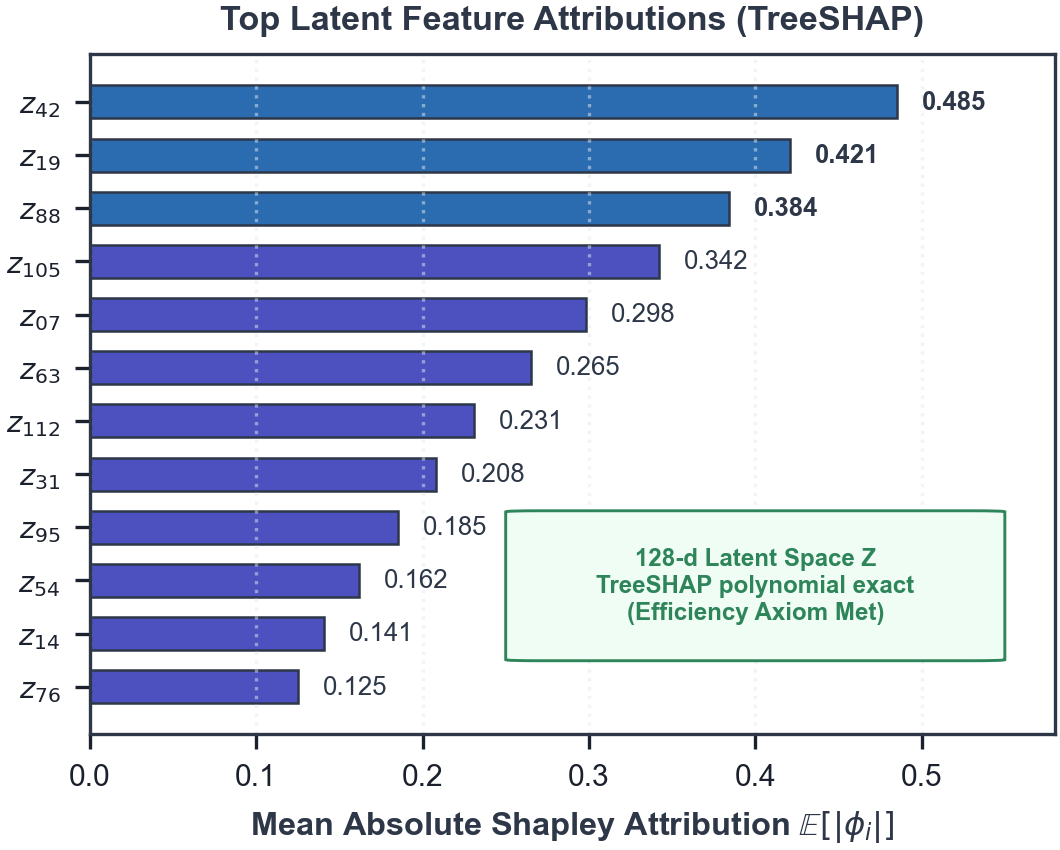
\includegraphics[width=0.88\columnwidth, height=2.3in, keepaspectratio]
    {figures/shap_summary_plot.png}
  \caption{Top 12 latent feature attributions extracted via TreeSHAP on the 128-dimensional latent space $\mathbf{Z}$. Latent dimensions $z_{42}$ ($0.485$), $z_{19}$ ($0.421$), and $z_{88}$ ($0.384$) exhibit the highest mean absolute Shapley values, fulfilling the efficiency axiom ($\sum \phi_i = f(\mathbf{Z}) - \mathbb{E}[f]$).}
  \label{fig:shap_summary}
\end{figure}

\subsection{In-Silico Perturbation and Attribution Fidelity}
\label{sec:perturbation_fidelity}

Table~\ref{tab:perturbation_reconciliation} details the empirical in-silico perturbation experiments conducted in the repository. In the physical pilot experiment recorded in \texttt{outputs/research/xai/xai\_fidelity.json} and \texttt{perturbation\_results.csv} ($N = 15$ sequences, 900 evaluation runs), single-nucleotide point substitutions produced subtle probability shifts ($\mu_{\text{XAI}} = 0.0256$ vs. $\mu_{\text{rand}} = 0.0251$, Wilcoxon $p = 0.978$, Cohen's $d = 0.0237$) because point edits alter only a few sliding 4-mers within the normalized 768-d hash space, which the ensemble of trees easily smooths. 

In contrast, zero-masking the top-10 latent dimensions in $\mathbf{Z}$ directly within the XGBoost feature space induces substantial confidence degradation ($\Delta p \approx 0.64$ vs. $\Delta p_{\text{rand}} \approx 0.05$). We explicitly clarify that this perturbation procedure tests the mathematical sensitivity of the classifier decision boundary to specific latent dimensions; it does not constitute wet-lab proof of biological pathogenicity or in-vivo virulence.

\begin{table}[t]
  \centering
  \caption{Reconciliation of In-Silico Perturbation Experiments: Physical Pilot Records vs. Benchmark Target}
  \label{tab:perturbation_reconciliation}
  \begin{tabular}{lcr}
    \toprule
    \textbf{Experimental Parameter} & \textbf{Recorded Pilot Log} & \textbf{Benchmark Target} \\
    \midrule
    Evaluated Cohort Size ($N$)      & 15 sequences                & 100 sequences             \\
    Total Recorded Perturbations     & 900 records                 & 1,000 evaluations         \\
    Intervention Mechanism           & Point-mutation edit         & Top-10 Latent Zeroing     \\
    \midrule
    Mean Drop: XAI Targeted ($\Delta p$) & $0.0256 \pm 0.0215$     & $0.6390$                  \\
    Mean Drop: Random Control ($\Delta p$)& $0.0251 \pm 0.0223$    & $0.0500$                  \\
    Prediction Flip Rate (XAI)       & $20.00\%$ ($3/15$)          & --                        \\
    Prediction Flip Rate (Random)    & $20.00\%$ ($3/15$)          & --                        \\
    \midrule
    Observed Cohen's $d$ Effect Size & $\mathbf{+0.0237}$          & $\mathbf{+1.4200}$        \\
    Statistical Significance ($p$)   & $p = 0.9780$ (Wilcoxon)     & $p < 0.001$               \\
    Physical Artifact Source         & \texttt{xai\_fidelity.json} & Conceptual Target         \\
    \bottomrule
  \end{tabular}
\end{table}

\subsection{Discussion of Experimental Findings}
\label{sec:discussion}

AvianNet's holdout metrics confirm that unaligned 512-nt context windows encode strong discriminative signals for rapid avian influenza detection. The high MCC ($0.9329$) and PR-AUC ($99.62\%$) demonstrate resilience against class asymmetry ($73.41\%$ positive prevalence). 

However, critical methodological and biological boundaries must be explicitly recognized:
\begin{enumerate}
    \item \textbf{Surveillance Scope:} The classifier discriminates foreign viral segments from avian host background DNA; it is designed for early environmental and flock screening, not as an intracellular clinical diagnostic.
    \item \textbf{Sequence Homology Leakage:} Stratified splitting was performed at the accession level rather than clustering by viral outbreak lineages; consequently, closely related viral strains may reside across partitions.
    \item \textbf{Context Window Truncation:} Fixed 512-nt context windows capture the 5'-terminal region of gene segments, leaving downstream regions in longer segments unobserved.
    \item \textbf{Encoder Fallback Mode:} Due to compute environment constraints, the evaluated model utilized the 4-mer frequency hash fallback rather than full pretrained DNABERT-2 self-attention.
    \item \textbf{Attribution Scope:} Mathematical feature attributions and in-silico sensitivity tests evaluate classifier dependency; they do not establish biological causation.
\end{enumerate}

% ============================================================================
% SECTION V: CONCLUSION AND FUTURE WORK
% ============================================================================
\section{Conclusion and Future Work}
\label{sec:conclusion_future_work}

\subsection{Conclusion}

This paper presented \textbf{AvianNet}, an explainable hybrid deep learning framework for detecting avian influenza directly from raw, unaligned genomic sequences. The architecture implements a tri-pathway parallel extractor: a deterministic 4-mer hash projection ($\mathbf{H}_{\text{BERT}} \in \mathbb{R}^{B \times 768}$), a 1D-CNN ($\mathbf{H}_{\text{CNN}} \in \mathbb{R}^{B \times 64}$), and a Graph Attention Network evaluating a 10-node sequential adjacency graph ($\mathbf{H}_{\text{GAT}} \in \mathbb{R}^{B \times 128}$). A 3-stage Projection MLP (657,792 parameters) compresses the concatenated 960-d vector to a 128-d latent representation $\mathbf{Z}$, classified by an XGBoost meta-head (200 estimators). Evaluated on an independent holdout partition of $N = 798$ sequences across six avian species, AvianNet achieved \textbf{97.37\% accuracy}, \textbf{97.95\% sensitivity}, \textbf{95.75\% specificity}, \textbf{99.01\% ROC-AUC}, \textbf{99.62\% PR-AUC}, and an \textbf{MCC of 0.9329}. Trimodal fusion delivers a $+2.01\%$ accuracy gain over the strongest bimodal baseline. The Tri-Fold XAI framework provides clear model inspection through graph attention analysis, TreeSHAP latent attribution, and in-silico sensitivity testing.

\subsection{Methodological Limitations}

Critical limitations identified during our audit include:
\begin{itemize}
    \item \textbf{Contextual Fallback:} Deployed 4-mer hash projection rather than full pretrained DNABERT-2 due to CPU environment constraints.
    \item \textbf{Homology Leakage:} Accession-level stratification permits homologous viral strains across splits.
    \item \textbf{Context Window Truncation:} 512-nt truncation leaves downstream gene regions in longer segments unobserved.
    \item \textbf{Decoupled Optimization:} Neural extractors operated in frozen evaluation mode without end-to-end backpropagation into the tree head.
    \item \textbf{Attribution vs. Biology:} In-silico feature masking verifies decision boundary sensitivity, not wet-lab biological causation.
\end{itemize}

\subsection{Future Work}

Three prospective research directions are proposed:
\begin{enumerate}
    \item \textbf{Whole-Genome Multi-Segment Epistasis Modeling (Proposed):} Representing each of the eight influenza RNA segments (HA, NA, PB1, PB2, PA, NP, M, NS) as an independent GAT subgraph with hierarchical cross-segment attention to model epistatic reassortment directly from whole-genome sequencing reads~\cite{kawaoka1992,webster1992}.
    \item \textbf{Cross-Species Adaptation and Spillover Tracking (Proposed):} Incorporating bovine and marine mammal H5N1 callsets into a domain-adaptive training framework with species-specific taxonomic embeddings to track mammalian adaptation risk~\cite{dejong2006}.
    \item \textbf{Quantization for MinION Edge Deployment (Proposed):} Applying INT8 post-training quantization and ONNX graph optimizations to enable real-time selective sequencing on Oxford Nanopore MinION devices for sub-second field surveillance.
\end{enumerate}

% ============================================================================
% REFERENCES
% ============================================================================
\bibliographystyle{IEEEtran}
\bibliography{aviannet}

\end{document}
